%! TeX program = lualatex
%---------------------------ALLGEMEINE IMPORTS-------------------------------------
\documentclass[12pt,english,ngerman]{scrartcl}
\input{protokoll_template/template.latex/input/shared_preamble.tex}

% Kopfzeile
\ihead{WS22\\
	17.05.2023}

\chead{\textsc{Stark} Matthias --- 12004907 \\
	\textsc{Philipp} Maximilian --- 11839611}

\ohead{FLAB 2 \\
Interferenz \\ und Polarisation}

% Fußzeile
%todo 
%\addbibresource{AdvancedMicroscopy.bib}

\usepackage{luacode}

\DeclareSIUnit\px{px}
\DeclareSIUnit\strich{|||}
\DeclareSIUnit\Var{var}
\DeclareSIUnit\VA{VA}
\DeclareSIUnit\bar{bar}

\usepackage{cleveref}

\crefname{enumerate}{Aufzählung}{Aufzählungen}

\begin{document}

\begin{luacode*}
dofile("createExtraPDF.lua")
\end{luacode*}

%
\includepdf{./deckblatt.pdf}
\tableofcontents

\newpage

\section{Aufgabenstellung}\label{Auf}

\subsection{Young'scher Doppelspalt, Beugungsgitter}

\begin{itemize}
	\item Bestimmen Sie das Beugungsmuster von vier Doppelspalten mit (bekannten) unterschiedlichen 
    Spaltbreiten und Spaltabständen. Berechnen Sie aus den Messwerten die Wellenlänge des Lasers.
	\item Erklären Sie die Details der beobachteten Beugungsmuster durch Vergleich mit den berechneten Mustern.
	\item Bestimmen Sie das Beugungsmuster eines Liniengitters und vergleichen Sie mit berechneten Werten. 
    Berechnen Sie aus den Messwerten die Gitterkonstante.
\end{itemize}

\subsection{Polarisation}

\begin{itemize}
	\item Verifizieren Sie das Gesetz von Malus.
	\item Untersuchen Sie den Einfluss des Durchlasswinkels eines weiteren Polarisators zwischen zwei gekreuzten Polarisatoren.
\end{itemize}

\subsection{Michelson Interferometer}

\begin{itemize}
	\item Justieren Sie das Interferometer und generieren Sie ein konzentrisches Interferenzmuster. 
    Bestimmen Sie durch Weglängenänderung die Wellenlänge 
    des Lasers. Wiederholen Sie dies für ein paralleles Interferenzmuster.
	\item Untersuchen Sie den absoluten Weglängenunterschied in den beiden Interferometerarmen, 
    sowie Auflösung und Stabilität des Interferometers.
	\item Untersuchen Sie die Rolle der Polarisation auf die Interferenzfähigkeit des Laserlichts.
\end{itemize}




\section{Grundlagen}\label{Grund}

%todo

Kohärenz

Die zeitliche Kohärenz bezieht sich auf den Grad der Ähnlichkeit zwischen zwei
Lichtwellen, die von derselben Quelle, aber zu unterschiedlichen Zeiten
ausgesendet werden. Lichtwellen bestehen aus oszillierenden elektrischen und
magnetischen Feldern, und damit es zu einer Interferenz kommt, müssen die
beiden Wellen eine konstante Phasenbeziehung haben. Das bedeutet, dass die
Phasendifferenz zwischen den beiden Wellen über einen längeren Zeitraum
konstant bleiben muss. Ändert sich die Phasenbeziehung schnell, wird von einer
geringen zeitlichen Kohärenz der Wellen ausgegangen. Bleibt die Phasenbeziehung
dagegen über einen langen Zeitraum konstant, so wird von einer hohen zeitlichen
Kohärenz ausgegangen.

Die räumliche Kohärenz hingegen bezieht sich auf den Grad der Ähnlichkeit
zwischen zwei Lichtwellen, die von derselben Quelle, aber an unterschiedlichen
Orten im Raum ausgesendet werden. Damit es zu einer Interferenz kommt, müssen
die beiden Wellen über ihre gesamte Wellenfront eine konstante Phasenbeziehung
aufweisen. Das bedeutet, dass die Phasendifferenz zwischen zwei beliebigen
Punkten der Wellenfronten konstant bleiben sollte. Wenn sich die
Phasenbeziehung über die Wellenfronten hinweg schnell ändert, wird von einer
geringen räumlichen Kohärenz der Wellen ausgegangen. Bleibt die Phasenbeziehung
dagegen über die Wellenfronten hinweg konstant, so wird von einer hohen
räumlichen Kohärenz ausgegangen.

Die Kohärenzlänge ist ein Maß dafür, wie weit sich das Licht unter Beibehaltung
seiner Kohärenz ausbreiten kann. Sie ist die Strecke, über die die
Phasenbeziehung zwischen zwei Punkten auf einer Wellenfront konstant bleibt.
Die Kohärenzlänge verhält sich umgekehrt proportional zur spektralen Bandbreite
der Lichtquelle. Eine schmalbandige Lichtquelle mit einer kleinen spektralen
Bandbreite hat eine große Kohärenzlänge, während eine breitbandige Lichtquelle
mit einer großen spektralen Bandbreite eine kleine Kohärenzlänge hat.

Zur Erzeugung von Interferenzmustern mit Licht ist eine Lichtquelle mit hoher
zeitlicher Kohärenz, hoher räumlicher Kohärenz und einer ausreichend langen
Kohärenzlänge erforderlich. Eine hohe zeitliche Kohärenz gewährleistet, dass
die Phasenbeziehung zwischen zwei Wellen über einen längeren Zeitraum konstant
bleibt, so dass sie konstruktiv oder destruktiv interferieren können. Eine hohe
räumliche Kohärenz stellt sicher, dass die Phasenbeziehung zwischen
verschiedenen Punkten auf den Wellenfronten konstant bleibt, so dass die Wellen
gleichmäßig über das Muster interferieren können. Die Kohärenzlänge bestimmt
die Größe des Bereichs, in dem Interferenz auftreten kann. Eine große
Kohärenzlänge ist notwendig, um gut definierte Interferenzstreifen zu
beobachten, während eine kurze Kohärenzlänge zu verschwommenen oder
verwaschenen Mustern führt.

% Young grundlagen

Das Youngsche Doppelspaltexperiment ist ein klassisches Experiment, das die
Wellennatur des Lichts und das Phänomen der Interferenz demonstriert. Dabei
wird Licht durch zwei eng beieinander liegende Spaltöffnungen geleitet und das
sich ergebende Muster auf einem hinter den Spaltöffnungen angebrachten
Bildschirm beobachtet.

Bei diesem Experiment wird eine kohärente Lichtquelle, z. B. ein Laser,
verwendet, um eine hohe zeitliche und räumliche Kohärenz zu gewährleisten. Das
Licht wird durch zwei schmale Schlitze geleitet, wodurch zwei
Lichtwellenquellen entstehen, die sich als halbkreisförmige Wellenfronten
ausbreiten. Diese Wellenfronten überlagern sich dann und interferieren
miteinander.

Um die Kriterien für konstruktive Interferenz im Young'schen
Doppelspaltexperiment zu verstehen, betrachten wir das Konzept der optischen
Wegdifferenz (OPD). Die OPD ist der Unterschied in der Strecke, die die
Lichtwellen von den beiden Spaltöffnungen bis zu einem bestimmten Punkt auf dem
Bildschirm zurücklegen. Wenn diese Differenz ein ganzzahliges Vielfaches der
Wellenlänge des Lichts ist, tritt an diesem Punkt konstruktive Interferenz auf.

Mathematisch lässt sich die Bedingung für konstruktive Interferenz wie folgt
ausdrücken:

% gleichung konstruktive Interferenzbedingung

wobei d der Abstand zwischen den beiden Schlitzen und θ der Winkel zwischen der
Verbindungslinie zwischen dem Punkt auf dem Schirm und den Schlitzen und der
Senkrechten zum Schirm ist.

Wenn die OPD gleich mλ ist, wobei m eine ganze Zahl ist, die die Ordnung des
Interferenzstreifens angibt, und λ die Wellenlänge des Lichts ist, tritt
konstruktive Interferenz auf. Das bedeutet, dass die Wellen der beiden Schlitze
an diesem Punkt des Schirms in Phase eintreffen, was zu einem hellen Streifen
führt.

Die quadrierte Amplitude der Welle steht in direktem Zusammenhang mit der
Lichtintensität, die an einem bestimmten Punkt des Bildschirms beobachtet wird.
Durch Quadrieren der Amplitude erhält man also das Interferenzmuster des
Doppelspalts. Das Muster besteht aus abwechselnd hellen und dunklen Streifen,
die als Interferenzstreifen oder -bänder bezeichnet werden.

% gleichung Doppelspalte

Zusätzlich zum Interferenzmuster des Doppelspalts wird jedoch noch ein weiteres
Interferenzmuster überlagert. Dieses zusätzliche Muster entsteht durch die
Interferenz von Lichtwellen, die durch jeden einzelnen Spalt laufen und sich
dann beugen, wodurch Einzelspalt-Interferenzmuster entstehen. Die einzelnen
Schlitze sind keine punktförmigen Quellen, und die gebeugten Wellen jedes
Spalts interferieren mit sich selbst.

Das Interferenzmuster der Einzelspalte ist durch ein zentrales Maximum und eine
Reihe kleinerer Maxima und Minima auf beiden Seiten gekennzeichnet. Dieses
Muster wird mit dem Interferenzmuster der Doppelspalte überlagert, wodurch sich
ein komplexeres Gesamtmuster ergibt, das auf dem Bildschirm zu sehen ist. Das
kombinierte Muster weist sowohl die Interferenzstreifen des Doppelspalts als
auch das Interferenzmuster des Einzelspalts auf.

% gleichung einzelspalt

Das im Young'schen Doppelspaltexperiment beobachtete Muster ist also die
Überlagerung von zwei Interferenzmustern: den Interferenzstreifen, die von den
Doppelspalten erzeugt werden, und dem Interferenzmuster, das sich aus der
Beugung der Einzelspalte ergibt. Dieses Experiment ist ein starker Beweis für
die Wellennatur des Lichts und das Phänomen der Interferenz.

% Malus gesetzt bitte verkuerzen
Das Gesetzt von Malus-Gesetz beschreibt die Beziehung zwischen der Intensität
des polarisierten Lichts, das durch einen Analysator übertragen wird, und dem
Winkel zwischen der Polarisationsrichtung des einfallenden Lichts und der
Übertragungsachse des Analysators.

Nach dem Malus-Gesetz ist die Intensität (I) des durchgelassenen Lichts gegeben
durch:

I = I₀ * cos²(θ)

wobei I₀ die anfängliche Intensität des einfallenden polarisierten Lichts und θ
der Winkel zwischen der Polarisationsrichtung des einfallenden Lichts und der
Transmissionsachse des Analysators ist.

Das Malus-Gesetz beruht auf dem Prinzip der Polarisation. Wenn unpolarisiertes
Licht einen Polarisator durchläuft, wird es polarisiert und seine elektrischen
Feldschwingungen auf eine bestimmte Richtung beschränkt. Das polarisierte Licht
ist durch seine Polarisationsrichtung gekennzeichnet, die senkrecht zur
Transmissionsachse des Polarisators verläuft.

Wenn das polarisierte Licht einen Analysator durchläuft, der ein weiterer
Polarisator mit einer bestimmten Transmissionsachse ist, hängt die Intensität
des übertragenen Lichts von der relativen Ausrichtung zwischen der
Polarisationsrichtung des einfallenden Lichts und der Transmissionsachse des
Analysators ab.

Wenn die Polarisationsrichtung des einfallenden Lichts perfekt mit der
Transmissionsachse des Analysators ausgerichtet ist (θ = 0), ist die
transmittierte Intensität (I) maximal und entspricht der Ausgangsintensität
(I₀).

Wenn der Winkel (θ) zwischen der Polarisationsrichtung des einfallenden Lichts
und der Transmissionsachse des Analysators zunimmt, nimmt die transmittierte
Intensität ab. Bei θ = 90 Grad ist die durchgelassene Intensität minimal und
wird zu Null. Dies ist der Fall, wenn die Polarisationsrichtung des
einfallenden Lichts senkrecht zur Transmissionsachse des Analysators steht.

Mathematisch gesehen zeigt das Malus-Gesetz, dass die übertragene Intensität
proportional zum Quadrat des Kosinus des Winkels zwischen der
Polarisationsrichtung und der Transmissionsachse ist. Mit zunehmendem Winkel
nimmt der Kosinus des Winkels ab, was zu einer Abnahme der übertragenen
Intensität führt.





\section{Versuchsanordnung}\label{sec:versuchsanordnung}

Für alle Versuche wird als Lichtquelle ein Laser mit einer Wellenlänge $\lambda$ von \SI{532}{\nano\meter} und einer 
Leistung von \SI{5}{\milli\watt} verwendet. Der gesamte Versuch wird auf einem Breadboard aufgebaut, welches auf einer 
gedämpften Steinplatte steht, um Erschütterungen besser ausgleichen zu können. Dies wird noch genauer in \autoref{sec:diskussion}
behandelt.
\subsection{Young'scher Doppelspalt, Beugungsgitter}

Der fertige Versuchsaufbau ist in \autoref{fig:aufbau_doppelspalt} sichtbar. Die entsprechenden Nummerierungen entsprechen dabei den 
Justierungsschritten in der Aufzählung.

\begin{enumerate}
    \item Zunächst wird der Laser am Breadboard parallel ausgerichtet. Dazu kann der Blechschirm mit der Skala (5) verwendet 
    werden. Zusätzlich kann damit der Laserstrahl während dem Hantieren oder Reflexionen ausgeblockt werden.
    \item Nun werden die beiden Spiegel, wie in \autoref{fig:aufbau_doppelspalt} sichtbar, aufgestellt, um den Laserstrahl 
    auf den entsprechenden Lichtweg zu lenken. Erneut ist die parallele Ausrichtung zu überprüfen.
    \item Nun wird mithilfe des entsprechenden Diahalters der Doppelspalt in den Lichtweg gegeben. Durch den Doppelspalt 
    entsteht eine Reflexion die auf den Spiegel zurückgeworfen wird. Durch die Position dieser Reflexion auf den Spiegel 
    kann die parallele Ausrichtung des Aufbaus überprüft werden. Nun werden die genauen Ausrichtungen der Spiegel und des 
    Lasers durch die entsprechenden Feinjustierungsschrauben so lange nachjustiert, bis die Positionen übereinstimmen.
    \item Um die Entfernung zwischen Schirm und Doppelspalt zu maximieren, wird als Schirm die Wand verwendet. Um die einzelnen 
    Distanzen zwischen den Beugungsmaxima besser bestimmen zu können, wird auf die Position des Beugungsbilds ein Blatt 
    Millimeterpapier geklebt.
\end{enumerate}

\begin{figure}[H]
	\begin{center}
		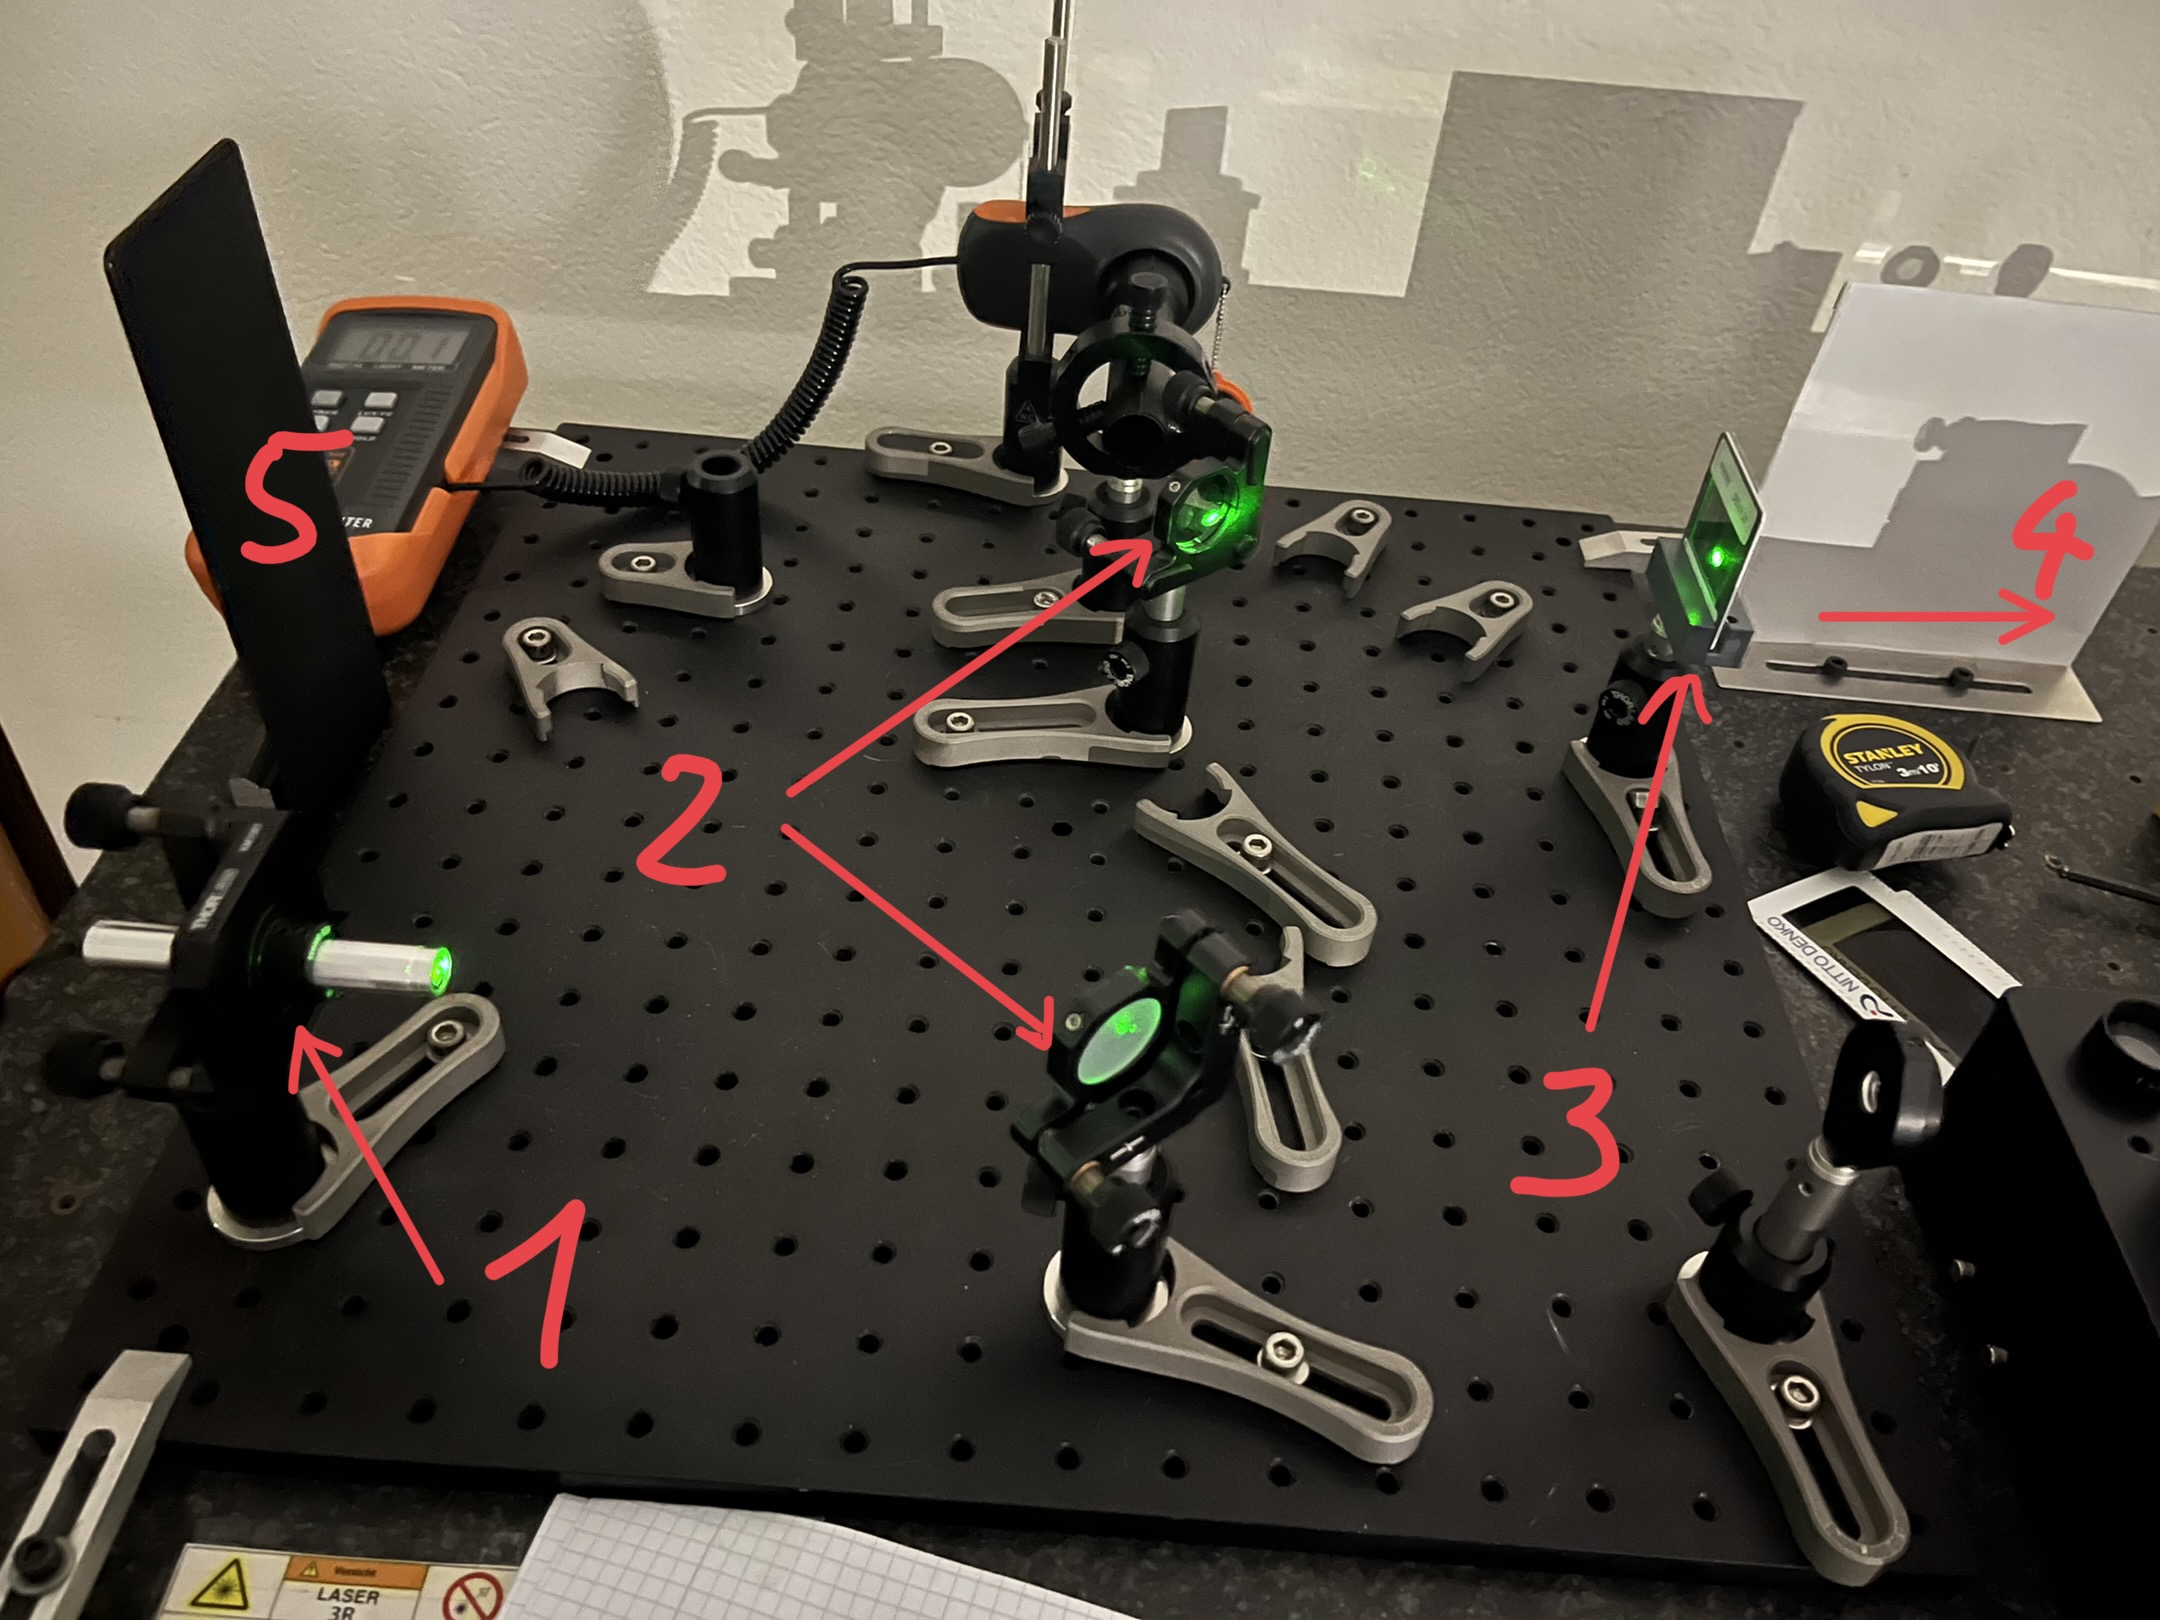
\includegraphics[width =0.75\textwidth]{./figures/aufbau_doppelspalt.jpg}
	\end{center}
	\caption[Versuchsaufbau für den Young'schen Doppelspalt und das Beugungsgitter] {
		Versuchsaufbau für den Young'schen Doppelspalt und das Beugungsgitter       \\
		1 \dots Laser                                    \\
		2 \dots Spiegel                                                      \\
		3 \dots Halterung mit Young'schen Doppelspalt oder dem Beugungsgitter                         \\
		4 \dots Schirm auf der Wand (nicht sichtbar) \\
		5 \dots Blechschirm mit Skala   
	}\label{fig:aufbau_doppelspalt}
\end{figure}

\subsection{Polarisation}

Der fertige Versuchsaufbau ist in \autoref{fig:aufbau_polarisation} sichtbar. Die entsprechenden Nummerierungen entsprechen dabei den 
Justierungsschritten in der Aufzählung.

\begin{enumerate}
    \item Zunächst wird wieder der Laser am Breadboard parallel ausgerichtet. Dabei kann der Blechschirm mit der Skala, 
    wie bereits erklärt verwendet werden.
    \item Nun wird ein Spiegel, wie in \autoref{fig:aufbau_polarisation} sichtbar, aufgestellt, um den Laserstrahl 
    zum Photodetektor (3) zu lenken. Erneut ist die parallele Ausrichtung zu überprüfen.
    \item Vor dem Photodetektor wird ein Rohr mithilfe einer entsprechenden Halterung befestigt, um die Hintergrundbeleuchtung
    möglichst abzuschirmen.
    \item Um die entsprechende Lichtintensität ablesen zu können, wird das entsprechende Messgerät mit dem Photosensor verbunden.
    \item Zwischen Photodetektor und Spiegel werden nun noch zwei Polarisationsfilter gegeben, deren Orientierung mit 
    einer Skala verbunden ist.
\end{enumerate}

\begin{figure}[H]
	\begin{center}
		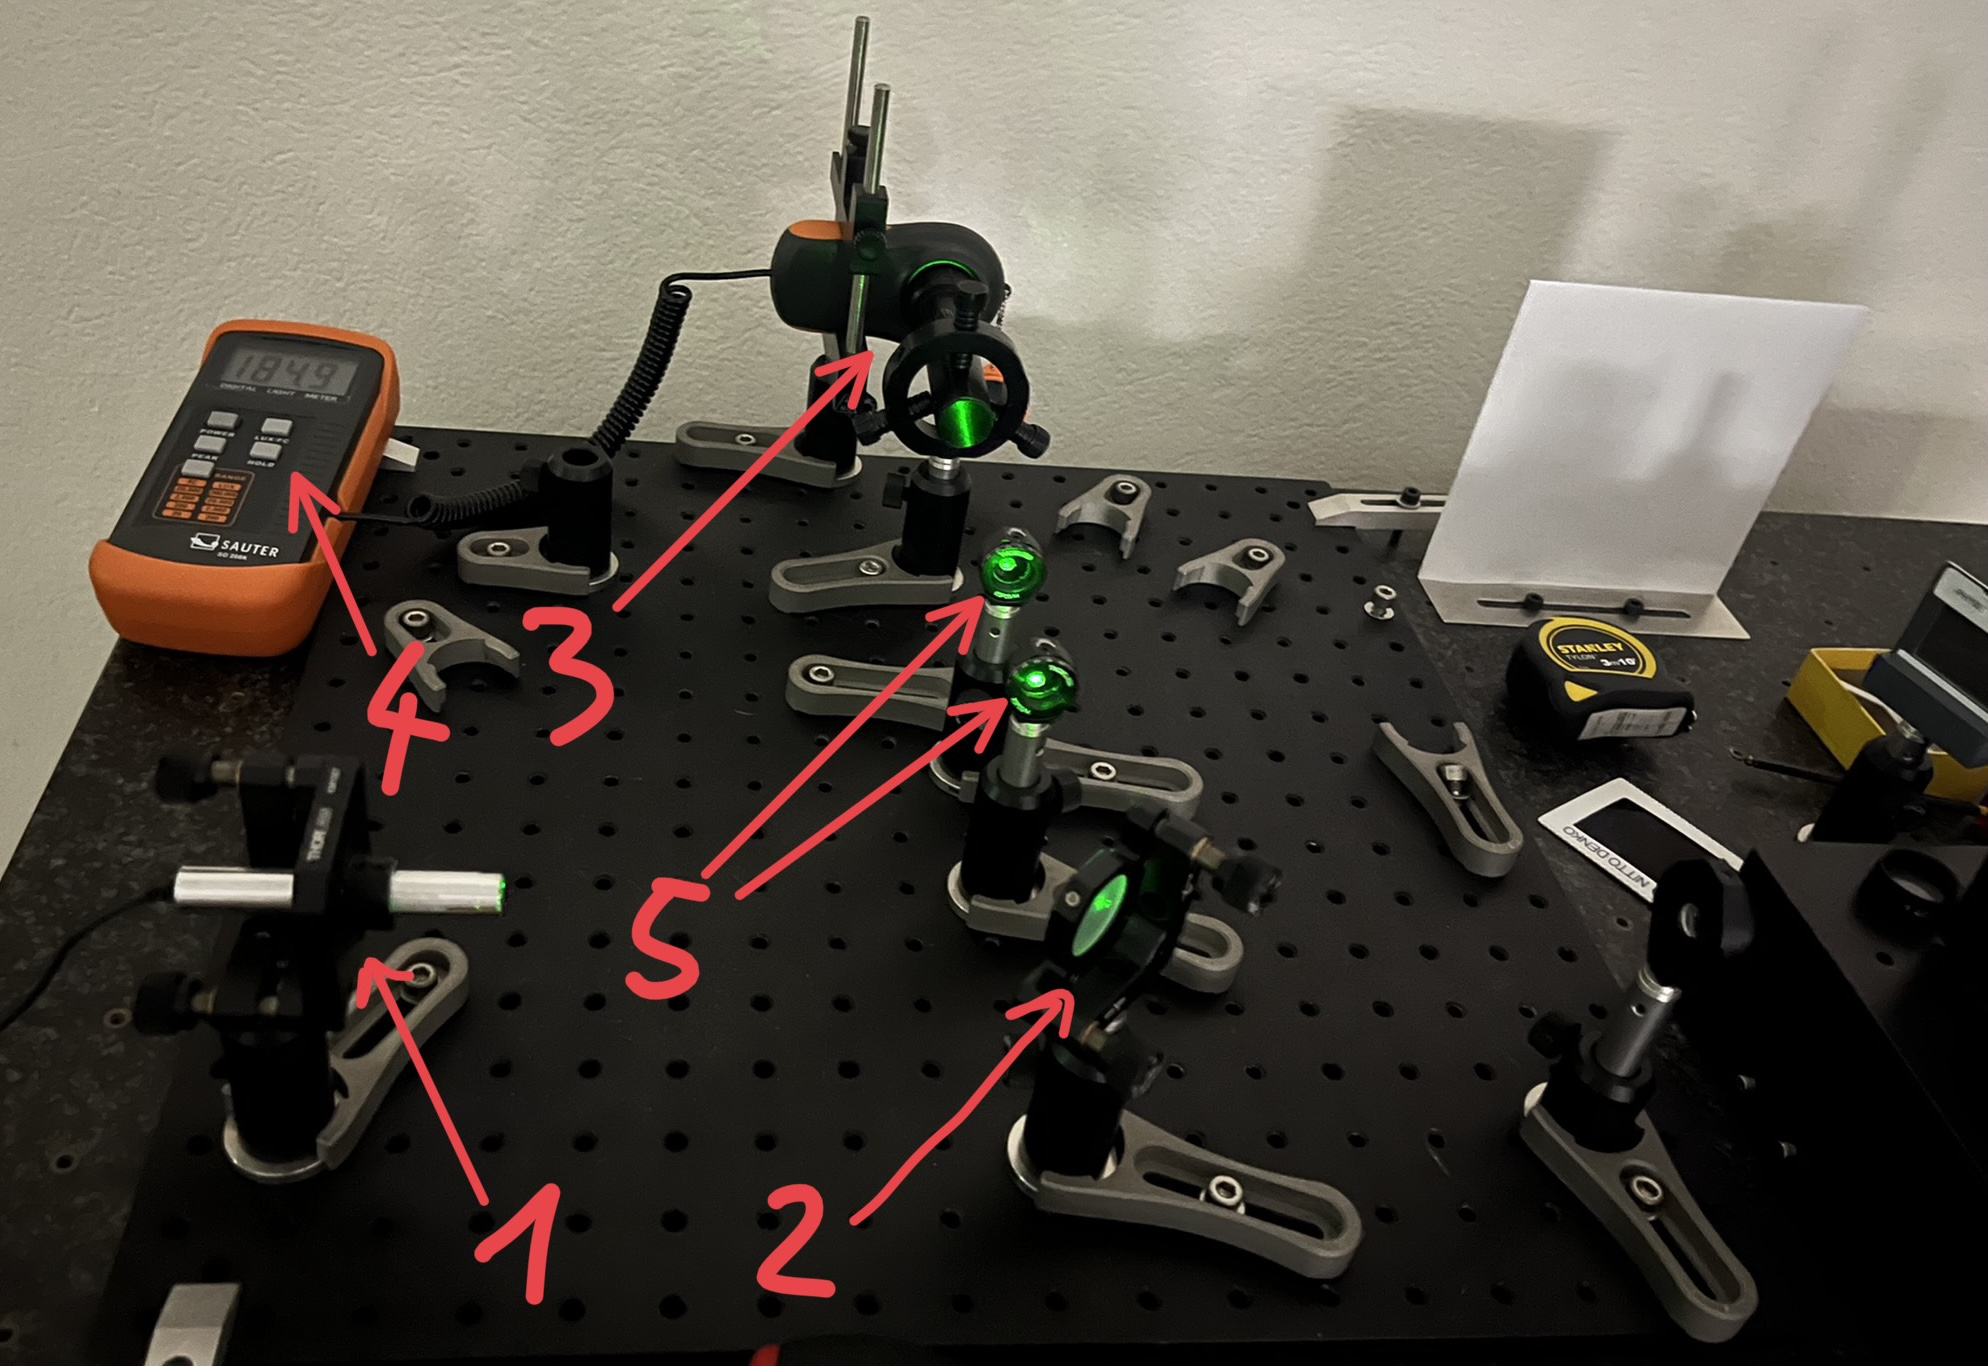
\includegraphics[width =0.75\textwidth]{./figures/aufbau_polarisation.jpg}
	\end{center}
	\caption[Versuchsaufbau für die Polarisation] {
		Versuchsaufbau für die Polarisation       \\
		1 \dots Laser                                    \\
		2 \dots Spiegel                                                      \\
		3 \dots Photodetektor mit Rohr                         \\
		4 \dots Messgerät für Photosensor \\
		5 \dots Polarisationsfilter   
	}\label{fig:aufbau_polarisation}
\end{figure}


\subsection{Michelson Interferometer}

Der fertige Versuchsaufbau ist in \autoref{fig:aufbau_interferometer} sichtbar. Die entsprechenden Nummerierungen entsprechen dabei den 
Justierungsschritten in der Aufzählung. Der Hauptbestandteil des Interferometers befindet sich nicht auf dem Breadboard,
sondern auf der Platte daneben.

\begin{enumerate}
    \item Zunächst wird die Platte, auf der sich das Interferometer befindet so befestigt, dass sie nicht mehr wackelt.
    \item Dann wird der Laser am Breadboard wieder parallel ausgerichtet, sodass dieser auf den Beamsplitter trifft.
    \item Der Strahlteiler sorgt dafür, dass der halbe Lichtstrahl durchgelassen und die andere Hälfte in einem Winkel
    von 90 ° abgelenkt wird.
    \item Nun Nun werden die beiden Spiegel so eingerichtet, dass das Licht zurück zum Beamsplitter geworfen wird, wo es 
    miteinander interferieren kann. Bei der genauen Ausrichtung der Spiegel ist dabei darauf zu achten, dass sich diese 
    im 90 ° Winkel zueinander befinden und beide Lichtwege ca. gleich lang sind.
    \item Am Schirm wird das Interferenzbild der beiden Laserstrahlen sichtbar. Die genaue Position des einen Spiegels 
    bzw. des Lasers muss nun so lange feinjustiert werden, bis ein Interferenzmuster sichtbar wird.
    \item Um dafür zu sorgen, dass das Interferenzmuster ringförmig wird, wird eine Linse in den Strahlengang vor den 
    Beamsplitter gegeben.
    \item Mit dieser Halterung kann im späteren Verlauf ein Polarisationsfilter im Strahlengang fixiert werden.
    \item Durch die Schraube und die entsprechende Übersetzung kann einer der beiden Lichtwege um eine kleine Distanz 
    verkürzt werden.
\end{enumerate}

\begin{figure}[H]
	\begin{center}
		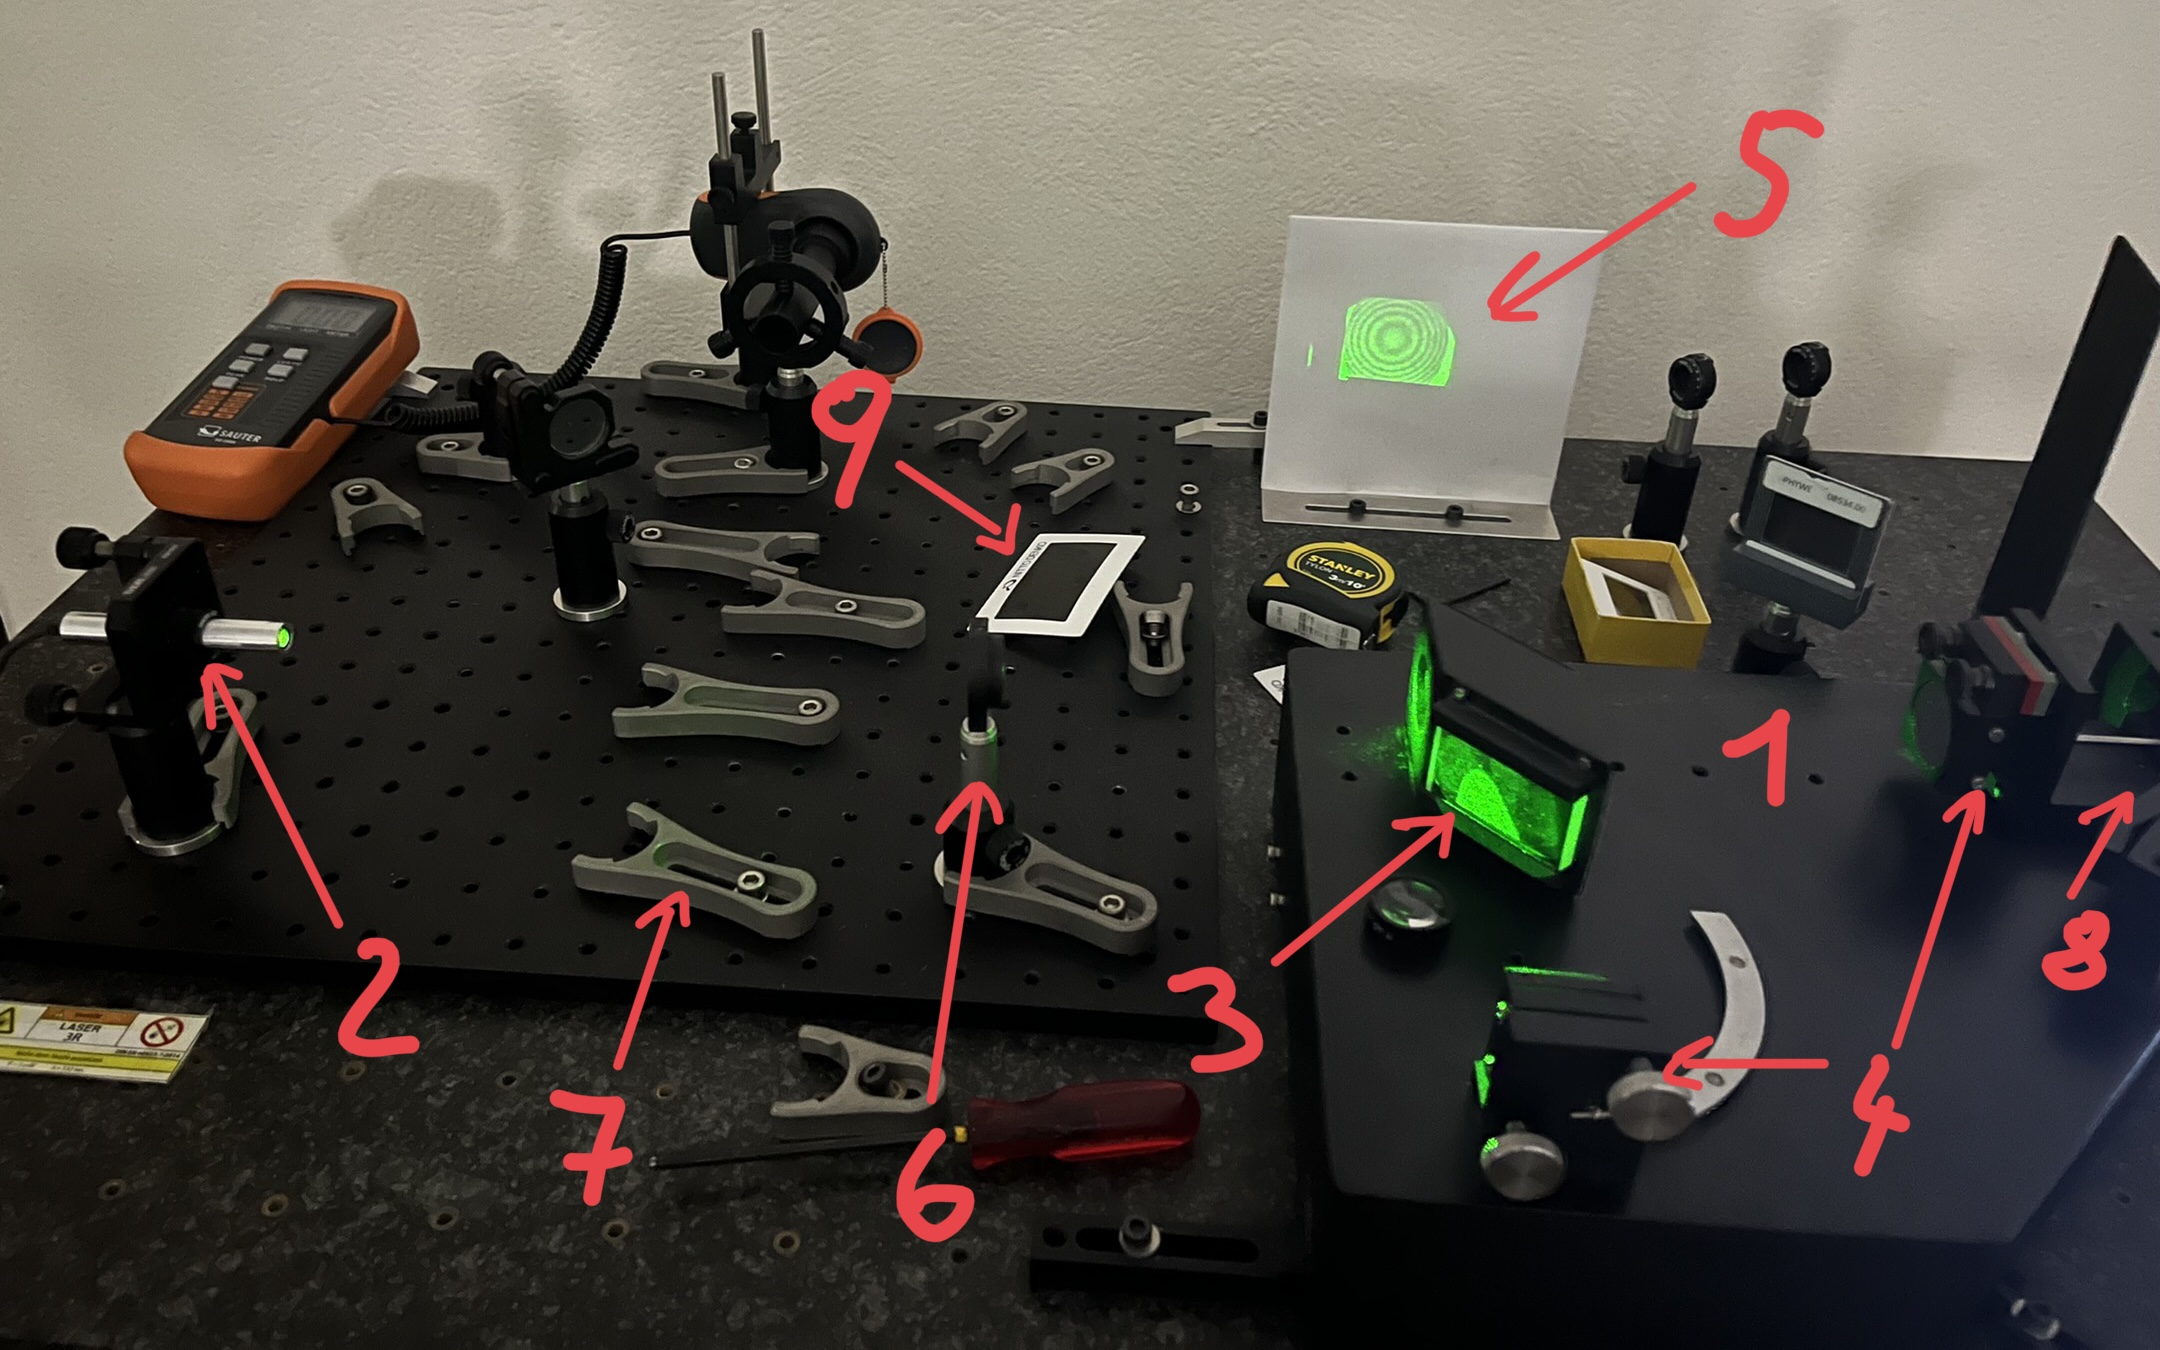
\includegraphics[width =0.75\textwidth]{./figures/aufbau_interferometer.jpg}
	\end{center}
	\caption[Versuchsaufbau für das Interferometer] {
		Versuchsaufbau für das Interferometer       \\
        1 \dots Platte für Interferometer                                    \\
		2 \dots Laser                                    \\
		3 \dots Beamsplitter                                                      \\
		4 \dots Spiegel                         \\
		5 \dots Schirm \\
		6 \dots Linse \\
        7 \dots Halterung für Polarisationsfilter \\
        8 \dots Schraube für die Distanzänderung der Lichtarme (nicht sichtbar) \\
        9 \dots Polarisationsfolie \\
	}\label{fig:aufbau_interferometer}
\end{figure}



\section{Geräteliste}\label{sec:geraeteliste}

Für den Versuch werden die in
\autoref{tab:gerate} aufgelisteten Geräte verwendet.

%todo

\begin{table}[H]
	\begin{center}
		\caption{Verwendete Geräte für die Abbildung durch eine Sammellinse
		}
		\begin{tblr}{cells={font=\footnotesize},colspec={lllll}}
			\textbf{Gerätetyp}               & \textbf{Hersteller} & \textbf{Typ} & \textbf{Anmerkung} \\
			Linse                            &                     &              & zu bestimmen       \\
			Lens Mount                       & ThorLabs            & LMR1/M       &                    \\
			Optical Posts                    & ThorLabs            & TR3          &                    \\
			Rail Carrier                     & ThorLabs            & XT34TR1/M    & 3x                 \\
			Halogenlampe                     & ThorLabs            & QTH10/M      &                    \\
			Mount for Rectangular Optics     & ThorLabs            & XYF1/M       &                    \\
			Resolution and Distortion Target & ThorLab             & R1L3S5P      &                    \\
			Aluminium-Schiene                &                     &              &                    \\
			Schirm                           &                     &              & selbst gebaut      \\
			Schibelehre                      & Workzone            & 819547       & digital            \\
		\end{tblr}\label{tab:gerate}
	\end{center}
\end{table}


\section{Versuchsdurchführung und Messergebnisse}\label{sec:versuchsdurchfuehrung_messergebnisse}

\subsection{Young'scher Doppelspalt, Beugungsgitter}

Zunächst muss der Versuchsaufbau, wie bereits in \autoref{sec:versuchsanordnung} beschrieben durchgeführt werden.
Nun werden der Reihe nach die 4 verschiedenen Doppelspalt in den Versuchsaufbau gegeben. Die entsprechenden Abmessungen der 
Doppelspalte sind dabei in \autoref{tab:masse_doppelspalt} sichtbar. Die entstehenden Beugungsmuster der einzelnen Doppelspalte werden dabei 
fotografiert und sind im Folgenden \autoref{fig:beugungsbild_spalt1} - \ref{fig:beugungsbild_spalt4} sichtbar. Um die entsprechenden Distanzen im Beugungsbild besser messen 
zu können, werden die so generierten Fotos bezüglich der Pixelpositionen genau ausgewertet, wie genauer in \autoref{sec:auswertung}
erklärt. Als Referenz dazu dient das im Hintergrund befindliche Millimeterpapier.



\begin{table}[H]
	\begin{center}
		\caption[Maße der Doppelspalte]{Maße der Doppelspalte mit implizit gegebener Unsicherheit \cite{unterlagen} \\
        $S_i$ \dots i-ter Doppelspalt \\
        $B$ \dots Spaltbreite in mm \\
        $D$ \dots Spaltabstand in mm
		}
		\begin{tblr}{cells={font=\footnotesize},colspec={lllll}}
			\textbf{}               & $B$ / mm & $D$ / mm  \\
			$S_1$                            & 0.10                    &   1.00                  \\
            $S_2$                            & 0.10                    &   0.50                  \\
            $S_3$                            & 0.10                    &   0.25                  \\
			$S_4$                            & 0.20                    &   0.25                  \\
		\end{tblr}\label{tab:masse_doppelspalt}
	\end{center}
\end{table}

Für das Fotografieren muss mit der Hintergrundbeleuchtung experimentiert werden, damit die Millimetereinteilung sichtbar ist,
jedoch auch die schwachen Beugungsordnungen noch erkannt werden können. Auch muss darauf geachtet werden, beim Aufnehmen der
Fotos möglichst nahe am Beugungsbild zu sein, aber keinen Zoom der Kamera zu verwenden, um eine mögliche Verzerrung auf den 
Bildern zu vermeiden. Auch sollten alle Fotos aus der gleichen Perspektive aufgenommen werden. Dazu wird ein kleines Gerüst
gebaut, um immer die gleiche Kameraposition zu treffen.

\begin{figure}[H]
	\captionbox{Erzeugtes Beugungsbild für Spalt 1 mit einer Spaltbreite von \SI{0.1}{\milli\meter} und einem Spaltabstand 
    von \SI{1}{\milli\meter}\label{fig:beugungsbild_spalt1}}{
		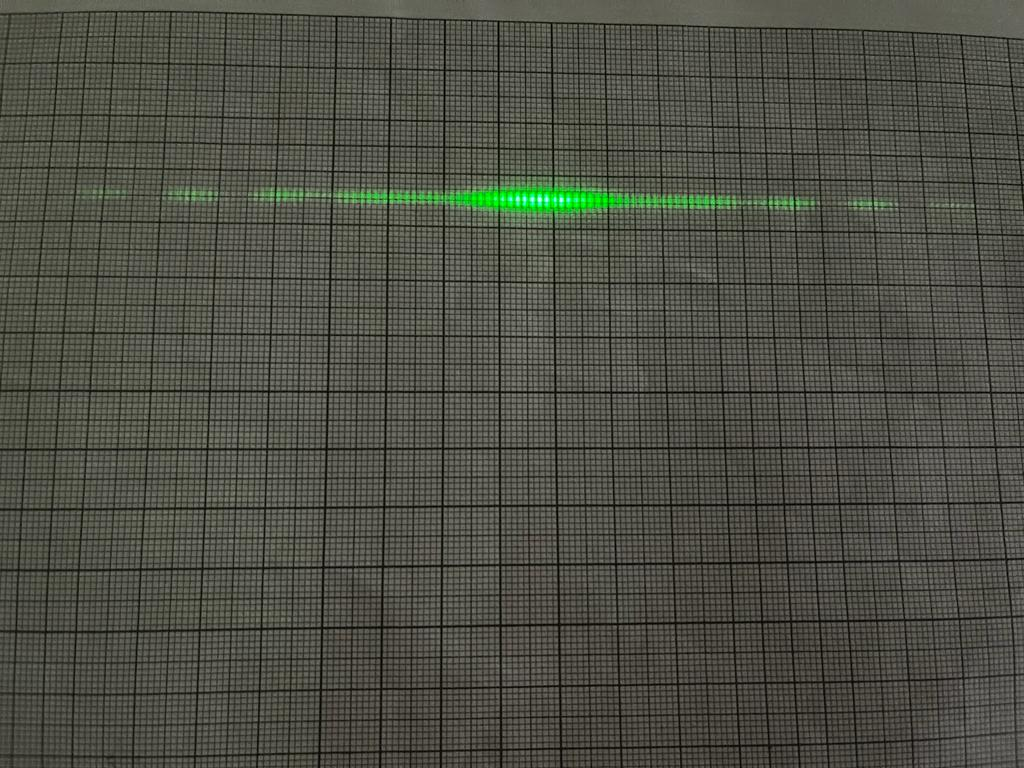
\includegraphics[width =.45\textwidth]{./figures/beugungsbild_spalt1.jpg} } \hfill
	\captionbox{Erzeugtes Beugungsbild für Spalt 2 mit einer Spaltbreite von \SI{0.1}{\milli\meter} und einem Spaltabstand 
    von \SI{0.5}{\milli\meter}\label{fig:beugungsbild_spalt2}}{
		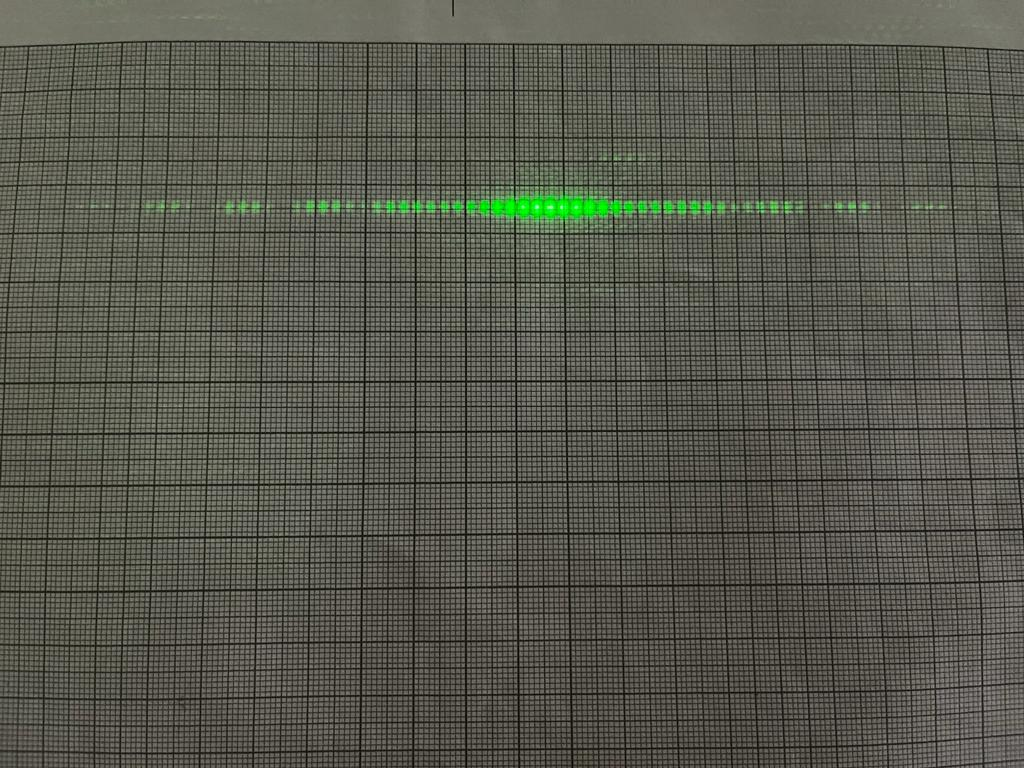
\includegraphics[width =.45\textwidth]{./figures/beugungsbild_spalt2.jpg}
	}

	\captionbox{Erzeugtes Beugungsbild für Spalt 3 mit einer Spaltbreite von \SI{0.1}{\milli\meter} und einem Spaltabstand 
    von \SI{0.25}{\milli\meter}\label{fig:beugungsbild_spalt3}}{
		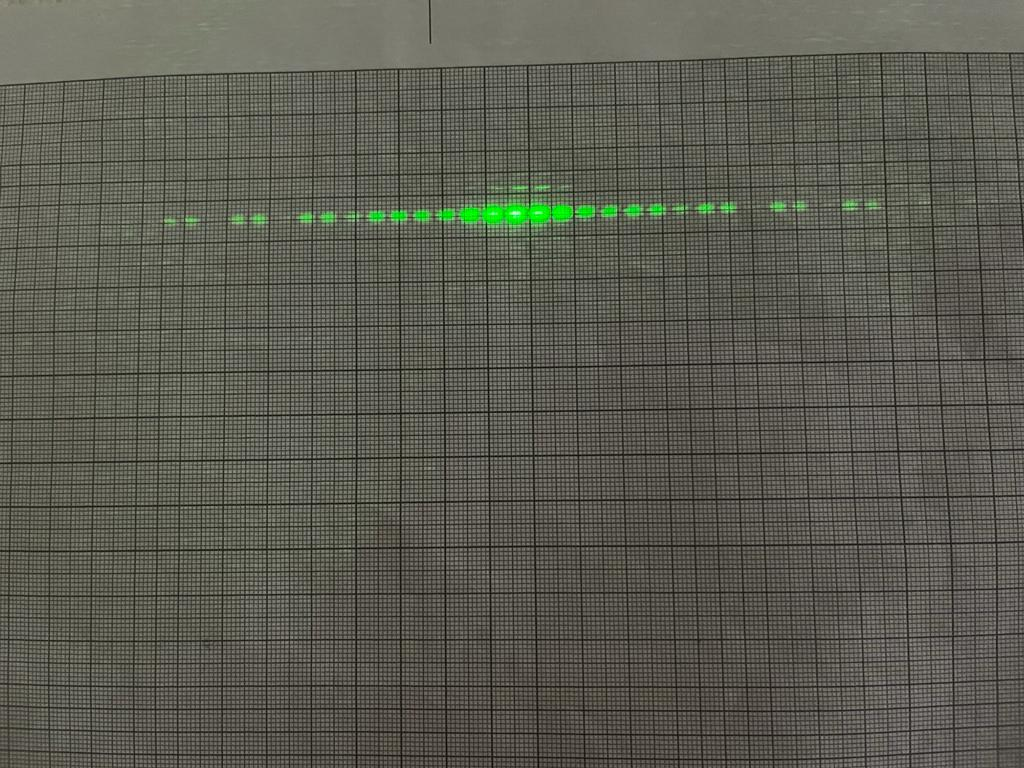
\includegraphics[width =.45\textwidth]{./figures/beugungsbild_spalt3.jpg} } \hfill
	\captionbox{Erzeugtes Beugungsbild für Spalt 4 mit einer Spaltbreite von \SI{0.2}{\milli\meter} und einem Spaltabstand 
    von \SI{0.25}{\milli\meter}\label{fig:beugungsbild_spalt4}}{
		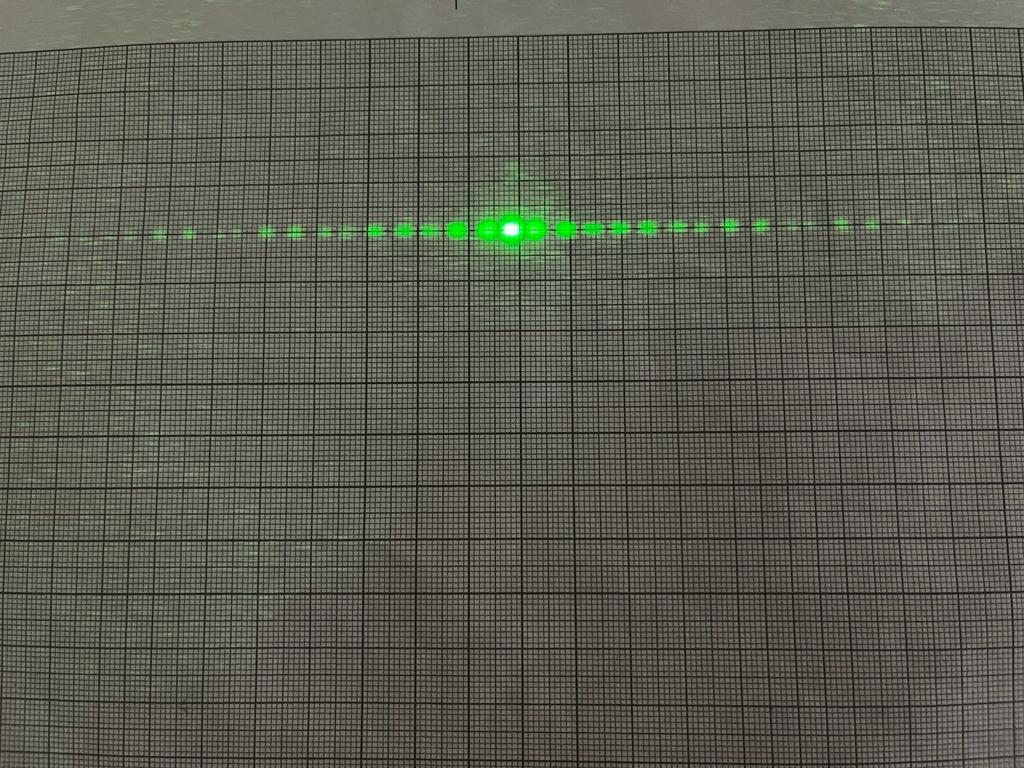
\includegraphics[width =.45\textwidth]{./figures/beugungsbild_spalt4.jpg} }
\end{figure}

Nun wird die Abdeckung mit den Doppelspalten durch ein Beugungsgitter, also viele, eng beieinander liegende Spalte ersetzt. 
Das so erzeugte Beugungsbild ist in \autoref{fig:beugungsbild_gitter} sichtbar.

\begin{figure}[H]
	\begin{center}
		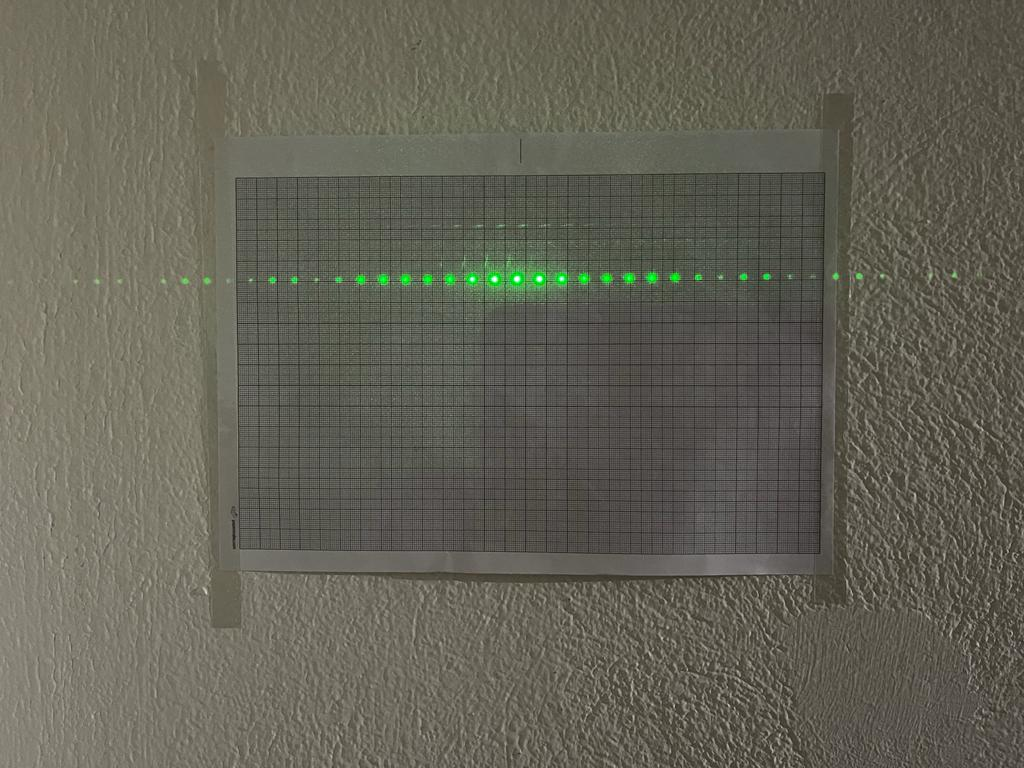
\includegraphics[width =0.5\textwidth]{./figures/beugungsbild_gitter.jpg}
	\end{center}
	\caption[ Erzeugtes Beugungsbild für das Beugungsgitter] {
        Erzeugtes Beugungsbild für das Beugungsgitter
	}\label{fig:beugungsbild_gitter}
\end{figure}


\subsection{Polarisation}

Zunächst muss der Versuchsaufbau, wie bereits in \autoref{sec:versuchsanordnung} beschrieben durchgeführt werden.

An beiden Polarisationsfiltern wird zunächst die 0-Position eingestellt und diese in den Aufbau gegeben.
Im verlauf des Versuchs sollen nun die Polarisationsebenen zueinander verdreht werden. Dazu bleibt ein Polarisationsfilter 
konstant in der gleichen Ausrichtung. Der andere Polarisationsfilter wird nun kontinuierlich weitergedreht und der 
abgelesene Skalenwert, sowie die gemessene Helligkeit in Lux am entsprechenden Photodetektor notiert, was in 
\autoref{tab:werte_polarisation} sichtbar ist. Am Messgerät ist dabei zu beachten, dass der kleinst mögliche Messbereich
gewählt wird. Die Unsicherheit des Winkel ist dabei so groß gewählt, weil der genaue Winkel recht schwer zu bestimmen war.
Auch ist darauf zu achten, die Raumbeleuchtung möglichst abzudunkeln, um die Messung dadurch nicht zu verfälschen.

%todo max tab:werte_polarisation

Zusätzlich wird auch der Intensitätswert ohne Polarisationsfilter, mit nur einem Filter und der Winkel bestimmt, an dem, 
laut Messgerät, kein Licht durch den Aufbau gelangt, gemessen und notiert.

%todo max bitte werte angeben

Nun wird noch ein dritter Polarisator in Form einer Polarisationsfolie in den Strahlengang gehalten durch den eigentlich keine
Intensität gelangt. Dabei werden folgende Werte erzeugt:

%todo max

Dabei sei angemerkt, dass nur so wenig Werte angegeben wurden, weil hier keine Gradmessung möglich war und der entsprechende 
Winkel nur geschätzt werden konnte.


\subsection{Michelson Interferometer}

Zunächst muss der Versuchsaufbau, wie bereits in \autoref{sec:versuchsanordnung} beschrieben durchgeführt werden.





\section{Auswertung}\label{sec:auswertung}

Um zu sehen wie sich die Unsicherheit der Messungen bis in die Ergebnisse
fortpflanzt, ist erweiterte Gauss-Methode verwendet worden. Die Grundlagen
dieser Methode stammen von den Powerpointfolien von
GUM~\cite{wolfgang_kessel_isobipm-gum_2004}. Für die Auswertung ist die
Progammiersprache Python im speziellen die Pakete \verb#labtool-ex2#,
\verb#pandas#, \verb#sympy#, \verb#lmfit# zur Hilfe genommen worden.
\verb#lmfit# wurde für das Fitten verwendet, \verb#sympy# wurde für symbolische
Manipulation verwendet und die restlichen Pakete für leichteres Handhaben der
Daten. Dies wurde aber alles durch \verb#labtool-ex2# abstrahiert.

Um höchstmögliche Genauigkeit zu garantieren wird erst bei der Darstellung der
Wert in Tabellen gerundet.

\subsection{Young'scher Doppelspalt, Beugungsgitter}

% Berechnen Sie die Beugungsmuster für die Doppelspalten 1-4 (die Spaltbreiten und -abstände sind in der Tabelle angegeben) und vergleichen Sie mit dem Experiment. Stellen Sie dazu jeweils einzeln den Interferenzterm und den Beugungsterm dar, sowie das gesamte Beugungsmuster. Vergleichen und erklären Sie auf Basis der berechneten Muster insbesondere die Lage der 1. Nebenmaxima der Doppelspalte 1 und 2.


% Vermessen oder fotografieren Sie das Beugungsmuster und bestimmen Sie die Gitterkonstante.
\subsection{Polarisation}

% Stellen Sie die winkelabhängige Transmission zusammen mit dem berechneten Verlauf graphische dar.

% Bringen Sie nun zwischen zwei gekreuzte Polarisatoren einen weiteren Polarisator ein (Polarisationsfolie). Beobachten Sie die jeweilige Transmission durch das Gesamtsystem und erklären Sie die Beobachtungen mit dem Gesetz von Malus.

\subsection{Michelson Interferometer}

\section{Diskussion}\label{sec:diskussion}

%todo dämpfung
\subsection{Young'scher Doppelspalt, Beugungsgitter}


\subsection{Polarisation}

Die beiden Polarisationsfilter werden auch außerhalb des Versuchsaufbaus vor eine Lichtquelle gehalten und 
zueinander verdreht. Dadurch wird festgestellt, dass die 0-Position an beiden Polaristatoren beinahe dazu führt, dass 
kein Licht durchgelangt. Dies deckt sich auch mit dem erzeugten Intensitätsverlauf in \autoref{fig:auswertung_polarisation}.

% bei 3 Polarisatoren gesetz von Malus
\subsection{Michelson Interferometer}

\section{Zusammenfassung}\label{sec:zusammenfassung}

Hier werden nochmals alle Ergebnisse dieser Experimentenfolge aufgelistet.
Wobei die meisten zu erstellenden Diagramme Aufgrund der Länge der
\autoref{sec:auswertung} entnommen werden sollen.

\subsection{Young'scher Doppelspalt, Beugungsgitter}


\subsection{Polarisation}


\subsection{Michelson Interferometer}


\newpage
\printbibliography
%todo literatur
\listoffigures
\listoftables
\end{document}